\chapter{Higher Ramification Group}
\label{cp:ramification}
\newtheorem{defi}{Definition}[chapter]
\newtheorem{rmk}{Remark}[chapter]
\providecommand*\thmautorefname{Theorem}

\section{Basic Ramification Theory}
In this section we define some basic concepts useful in analyzing how prime behaves while moving along algebra extensions. Main result are \autoref{thm:thm-22} and \autoref{thm:thm-24}.
\begin{defi}[Residue field]
    ~\begin{itemize}
        \item \textbf{Residue field} $k(\mathfrak{p})$ at prime ideal $\mathfrak{p}$ in a general Dedekind domain $A$: $A/\mathfrak{p}$
        \begin{listing}[!htpb]
        \begin{minted}{lean}
def LocalRing.ResidueField (R : Type u_1) [CommRing R] [LocalRing R] : Type u_1 :=
    R / LocalRing.maximalIdeal R
        \end{minted}
        \end{listing}
    \end{itemize}
\end{defi}
\begin{rmk}
    In the first glimpse, the definition in Lean is very different from our definition. But in fact Lean's definition is more general. \\
    It can be proved that for general ring $A$ and its prime ideal $\mathfrak{p}$,
    \begin{equation}
        \notag
        Frac(A/\mathfrak{p}) \simeq A_{\mathfrak{p}} / \mathfrak{p} A_{\mathfrak{p}}
    \end{equation}
    where $A_{\mathfrak{p}}$ is a localization.
    In our case, take $A$ a Dedekind domain, so $\mathfrak{p}$ is a maximal ideal, hence $Frac(A/\mathfrak{p})$ is just $A/\mathfrak{p}$. Therefore,
    \begin{equation}
        \notag
        k(\mathfrak{p}) \simeq \verb|LocalRing.ResidueField | A_{\mathfrak{p}}
    \end{equation}
\end{rmk}
\begin{rmk} More on residue field
~\begin{itemize}
    \item [] The residue field at a prime $\mathfrak{p}$ is essentially the field you get by "modding out" by $\mathfrak{p}$. This operation simplifies the arithmetic and focuses on the essential behavior of that prime. Normally, we don't care much about what happends within the ideal $\mathfrak{p}$, rather, we study how $\mathfrak{p}$ behaves as a whole.
\end{itemize}
\end{rmk}
\noindent
%In the following part of this section, we admits the following setup here:
% \begin{equation}
%     \notag
%     \begin{matrix}
%     \begin{tikzpicture}[node distance=1.5cm, auto]
%     \node (L) {$L$};
%     \node (K) [below of=L] {$K$};
%     \node (A) [below of=K] {$A$ (Dedekind)};
%     \node (B) [left of=K, above=0.5cm] {$B$};

%     \draw[-] (L) -- node[right] {fin deg, separable} (K);
%     \draw[-] (K) -- node[right] {field of fractions} (A);
%     \draw[-] (B) to [out=-90,in=160] node[left, xshift=0.5cm] {integral closure} (A);
%     \end{tikzpicture} &
%     \begin{tikzpicture}[node distance=1.5cm, auto]
%     \node (L) {$L$ (number field)};
%     \node (K) [below of=L] {$\mathbb{Q}$};
%     \node (A) [below of=K] {$\mathbb{Z}$};
%     \node (B) [left of=K, above=0.5cm] {$\mathcal{O}_L$};

%     \draw[-] (L) -- node[right] {fin deg, separable} (K);
%     \draw[-] (K) -- node[right] {field of fractions} (A);
%     \draw[-] (B) to [out=-90,in=160] node[left, xshift=0.5cm] {integral closure} (A);
%     \end{tikzpicture}
%     \end{matrix}
% \end{equation}
%\newpage
%\begin{figure}[!htpb]
%\centering
%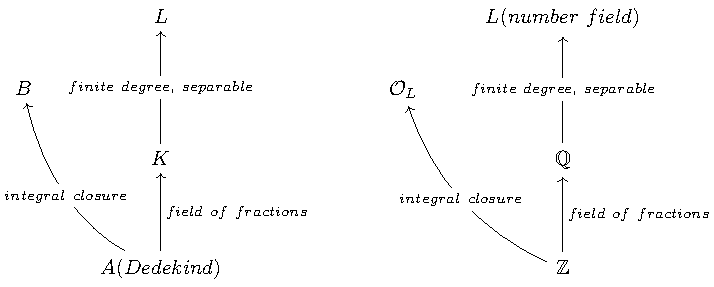
\includegraphics[width=\linewidth]{Figures/figure1.pdf}
%\end{figure}
%\noindent
%Where $A$ is a Dedekind domain with field of fractions $K$, and $B$ the integral closure of $A$ in a finite separable extension $L$ of $K$. In particular, when only number field is concerned, we have the right diagram.
%\begin{thm}
%    $B$ is a Dedekind domain. \rm{(For proof see ANT. Theorem 3.29.)}
%    \begin{listing}[!htpb]
%    \begin{minted}{lean}
%theorem IsIntegralClosure.isDedekindDomain (A : Type u_2) (K : Type u_3) [CommRing A] [Field K] [Algebra A K] [IsFractionRing A K] (L : Type u_4) [Field L] (C : Type u_5) [CommRing C] [Algebra K L] [Algebra A L] [IsScalarTower A K L] [Algebra C L] [IsIntegralClosure C A L] [Algebra A C] [IsScalarTower A C L] [FiniteDimensional K L] [IsDomain A] [Algebra.IsSeparable K L] [IsDomain C] [IsDedekindDomain A] :
%    IsDedekindDomain C
%    \end{minted}
%    \end{listing}
%\end{thm}
\noindent
Now consider $A$ a Dedekind domain with field of fractions $K$, and $B$ the integral closure of $A$ in a finite separable extension $L$ of $K$. $\mathfrak{p}$ is a prime ideal of $A$, it generates an ideal $\mathfrak{p}B$ in $B$. In particular, if only number field is concerned, $A, \ B, \ K$ are $\mathbb{Z}, \ \mathcal{O}_L, \ \mathbb{Q}$ respectively. We visualize our setup as below.
\newline
% \begin{center}
%     \begin{tikzpicture}[node distance=2cm, auto]
%     \node (L) {$L$};
%     \node (K) [below of=L] {$K$};
%     \node (A) [below of=K] {$A$ (Dedekind)};
%     \node (B) [left of=K, above=0.5cm] {$B$};
%     \node (P) [left of=B] {$\mathfrak{p}B$};
%     \node (p1) [left of=A] {};
%     \node (p) [left of=p1] {$\mathfrak{p}$};

%     \draw[-] (L) -- node[right] {finite degree, separable} (K);
%     \draw[-] (K) -- node[right] {field of fractions} (A);
%     \draw[-] (B) to [out=-90,in=160] node[above] {integral closure} (A);
%     \draw[-] (p) -- node[below] {prime ideal} (A);
%     \draw[-] (P) -- node[above] {ideal} (B);
%     \draw[->] (p) -- node[left] {generates} (P);
% \end{tikzpicture}
% \end{center}
\begin{figure}[!htpb]
\centering
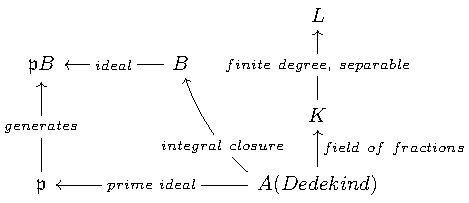
\includegraphics[width=0.7\linewidth]{Figures/figure2.pdf}
\end{figure}
\noindent
$B$ is a Dedekind domain (see ANT.Theorem 3.29), then by the factorization of ideals in Dedekind domain (see \verb|Ideal.uniqueFactorizationMonoid|), $\mathfrak{p}B$ factors into:
\begin{equation}
    \notag
    \mathfrak{p}B=\mathfrak{P}_1^{e_1} \dots \mathfrak{P}_g^{e_g}
\end{equation}
where $\mathfrak{P}_i$ are prime ideals in $B$.
\begin{defi}[Lies over]
    ~\begin{itemize}
        \item $\mathfrak{P}$ \textbf{lies over} $\mathfrak{p}$: $\mathfrak{P}$ appears in the factorization of $\mathfrak{p}$.
    \end{itemize}
\end{defi}
\begin{rmk}
    One may also say that $\mathfrak{P}$ divides $\mathfrak{p}$ here. In Lean, there is no explicit definition of it, but one can still use \verb|map f p| \ $\leq$ \ \verb|P| (where \verb|f : R →+* S|) to indicate the same thing.
\end{rmk}
\begin{defi}[Ramified]
    ~\begin{itemize}
        \item $\mathfrak{p}$ is \textbf{ramified} in $B$ (or $L$): if any of the $e_i$ is $\geq 2$.
        \item (\textbf{Unramified}: all $e_i$ are 1. Also, we say the field $L$ is ramified when there exists a ramified prime ideal of $A$, otherwise it is unramified)
    \end{itemize}
\end{defi}
\begin{defi}[Ramification index]
    ~\begin{itemize}
        \item \textbf{Ramification index} $e(\mathfrak{P}/\mathfrak{p})$: the power of $\mathfrak{P}$ in the factorization of $\mathfrak{p}$. e.g., $e(\mathfrak{P}_i/\mathfrak{p})=e_i$.
        \begin{listing}[!htpb]
        \begin{minted}[escapeinside=--,mathescape=true]{lean}
noncomputable def Ideal.ramificationIdx {R : Type u} [CommRing R] {S : Type v} [CommRing S] (f : R →+* S) (p : Ideal R) (P : Ideal S) :-$\mathbb{N}$- := 
    sSup {n | map f p -$\leq$- P -$\wedge$- n}
        \end{minted}
        \end{listing}
    \end{itemize}
\end{defi}
\begin{rmk}
    In Lean, ramification index is defined with respect to all ideals and all commutative rings, it is the largest exponent $e$ such that $\mathfrak{p}$ is contained in $\mathfrak{P}^e$. In particular, if $\mathfrak{p}$ is not contained in any $\mathfrak{P}^e$, then the ramification index is 0. If there is no largest such $e$ (like when $\mathfrak{p}$ is trivial), then it is also defined to be 0.
\end{rmk}
\begin{rmk}
Understanding ramification more deeply:
\begin{itemize}
    \item[] When we "move" a prime ideal of a domain into a larger domain, ramification helps us to determine whether it behaves well. Four things can happend here:
    \begin{enumerate}
        \item it stays as a single prime ideal. (unramified)
        \item it splits into distinct primes. (unramified)
        \item it stays as a single prime but with a higher exponent. (totally ramified)
        \item it splits into several primes, some of which have higher exponents. (ramified)
    \end{enumerate}
    Obviously the prime behaves more complicated and "badly" in the last two situations - we name this "ramified". A ramified prime acts "badly", but how bad? Then it comes to tamely/wildly ramification.
\end{itemize}
\end{rmk}
\begin{thm}
    \label{tab:thm-21}
    If $L$ is Galois over $K$, then all the ramification indexes (of primes lying over $\mathfrak{p}$) are equal and all the residue class degrees are equal. Further, $efg=[L : K]$. (See ANT. Theorem 3.34 for proof.)
\end{thm}
\begin{defi}[Tamely and wildly ramified]
~\begin{itemize}
    \item $\mathfrak{P}/\mathfrak{p}$ is \textbf{tamely ramified}: ramification index $e(\mathfrak{P}/\mathfrak{p})$ is relatively prime to the characteristic of residue field $k(\mathfrak{P})$.
    \item (\textbf{wildly ramified}: otherwise.)
\end{itemize}
\end{defi}
%\begin{defi}[Inertial degree]
%    ~\begin{itemize}
%        \item \textbf{Inertial degree} $f(\mathfrak{P}_i/\mathfrak{p})$ of $\mathfrak{P}_i$ over $\mathfrak{p}$: the degree of field extension $[k(\mathfrak{P}_i) : k(\mathfrak{p})]$
%        \begin{listing}[!htpb]
%        \begin{minted}[escapeinside=||,mathescape=true]{lean}
%noncomputable def Ideal.inertiaDeg {R : Type u} [CommRing R] {S : Type v} [CommRing S] (f : R →+* S) (p : Ideal R) (P : Ideal S) [p.IsMaximal] :|$\mathbb{N}$|
%        \end{minted}
%        \end{listing}
%    \end{itemize}
%\end{defi}
\begin{thm}
    \label{thm:thm-22}
    If $B$ is a free $A$-module, then prime $\mathfrak{p}$ ramifies in $L$ iff $\mathfrak{p} \mid disc(B/A)$. In particular, only finitely many prime ideals ramify. \rm{(See ANT. Theorem 3.35 for proof.)}
\end{thm}
\begin{thm}[Hermite]
    \label{thm:thm-23}
    Every nontrivial number field has discriminant greater than 2. \rm{(This is a direct collary of ANT. Theorem 4.3.)}
    \begin{listing}[!htpb]
    \begin{minted}[escapeinside=--,mathescape=true]{lean}
theorem NumberField.abs_discr_gt_two {K : Type u_1} [Field K] [NumberField K] (h : 1 < FiniteDimensional.finrank-$\mathbb{Q}$- K) : 2 < |NumberField.discr K|
    \end{minted}
    \end{listing}
\end{thm}
\begin{thm}[Minkowski]
    \label{thm:thm-24}
Every nontrivial number field is ramified.\rm{(there must be a prime $p \in \mathbb{Z}$ ramifies in the extension.)}
\begin{proof}
This is a direct result of \autoref{thm:thm-22} and \autoref{thm:thm-23}.
\end{proof}
\end{thm}
\newpage
\section{Higher Ramification Group}
Previous section provides us with initial concepts to study prime's behaviour. But ramified/unramified is a rough classification, we often need more delicate analysis. That's when higher ramification group comes into play. \\
We now focus on number fields. Suppose the following setup:
% \begin{center}
% \begin{tikzpicture}[node distance=2cm, auto]
%     \node (K) {$K$};
%     \node (Q) [below of=K] {$\mathbb{Q}$};
%     \node (A) [left of=K] {$\mathcal{O}_K$};
%     \node (p) [left of=A] {$\mathfrak{p}$};
%     \node (Z) [left of=Q] {$\mathbb{Z}$};
%     \node (p') [left of=Z] {$(p)$};

%     \draw[-] (K) -- node[right] {finite degree} (Q);
%     \draw[-] (K) -- (A);
%     \draw[-] (A) -- node[above] {prime} (p);
%     \draw[-] (Q) -- (Z);
%     \draw[-] (Z) -- node[above] {prime} (p');
%     \draw[->] (p) -- node[left] {lies over} (p');
% \end{tikzpicture}
% \end{center}
\begin{figure}[!htpb]
\centering
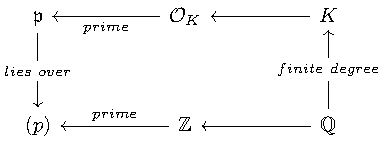
\includegraphics[width=0.6\linewidth]{Figures/figure3.pdf}
\end{figure}
\noindent
\begin{defi}[Decomposition group and decomposition field]
    ~\begin{itemize}
        \item \textbf{Decomposition group} $D(\mathfrak{p}/p)$: the stabilizer of $\mathfrak{p}$ under action of $Gal(K/\mathbb{Q})$. i.e., \\
        $\{ \sigma \in Gal(K/\mathbb{Q}) \mid \sigma(\mathfrak{p}) = \mathfrak{p}\}$.
        \item \textbf{Decomposition field}: fixed field of $D(\mathfrak{p}/p)$, denoted $\mathcal{F}_K (D(\mathfrak{p}/p))$.
        \begin{listing}[!htpb]
        \begin{minted} [escapeinside=``]{lean}
@[reducible, inline]
abbrev ValuationSubring.decompositionSubgroup (K : Type u_1) {L : Type u_2} [Field K] [Field L] [Algebra K L] (A : ValuationSubring L) : Subgroup (L`$\simeq_{\rm a}$`[K] L) :=
    MulAction.stabilizer (L `$\simeq_{\rm a}$`[K] L) A
        \end{minted}
        \end{listing}
    \end{itemize}
\end{defi}
\begin{rmk} Similar to residue field, we investigate $\mathfrak{p}$ as a whole here. Thus $\sigma \in D(\mathfrak{p}/p)$ might permutes elements in $\mathfrak{p}$, but it must fix $\mathfrak{p}$ as a whole. \\Lean defines decomposition group to be the stabilizer of the action on the type of all valuation subrings of the field, where valuation subring of a field $L$ is a subring $A$ such that for every $x \in L$, either $x \in A$ or $x^{-1} \in A$. \\These two definitions are not exactly the same. But the stabilizer of $A$ is the same as the stabilizer of the maximal ideal $\mathfrak{m}$ of $A$, i.e.,
    $\{\sigma \in Gal(L/K) \mid \sigma(A) = A\} = \{\sigma \in Gal(L/K) \mid \sigma(\mathfrak{m}) = \mathfrak{m}\}$.
Hence we shall obtain the same thing by substituting $A$ with $(\mathcal{O}_K)_\mathfrak{p}$.\\
Technically, one can create a prime spectrum by \verb|IsDedekindDomain.HeightOneSpectrum| with desired prime and use \verb|IsDedekindDomain.HeightOneSpectrum.valuation| to get a valuation attached to the ideal. Finally \verb|Valuation.valuationSubring| can transform it into a valuation subring, then we can plug it into \verb|ValuationSubring.decompositionSubgroup|.
\end{rmk}
\noindent
Since $\sigma \in D({\mathfrak{p}}/p)$ sends $\mathfrak{p}$ to itself, a natural automorphism emerges here:
\begin{equation}
    \notag
    \sigma' : \ k(\mathfrak{p}) \longrightarrow k(\mathfrak{p}), \ x \ mod \ \mathfrak{p} \longmapsto \sigma(x) \ mod \ \mathfrak{p}
\end{equation}
$D({\mathfrak{p}}/p) \leq Gal(K/\mathbb{Q})$, so $\sigma$ fixes $\mathbb{Q}$, hence $k(p)$.
Consider group homomorphism:
\begin{equation}
    \notag
    D({\mathfrak{p}}/p) \longrightarrow Gal(k(\mathfrak{p}) / k(p)), \ 
    \sigma \longmapsto \sigma'
\end{equation}
\begin{defi}[Inertia group]
~\begin{itemize}
    \item \textbf{inertia group} $I(\mathfrak{p}/p)$ of $\mathfrak{p}$: the kernel of this homomorphism. i.e., \\$\{\sigma \in D(\mathfrak{p}/p) \mid \forall x \in \mathcal{O}_K, \ \sigma(x) \equiv x \ mod \ \mathfrak{p}\}$
    \begin{listing}[!htpb]
    \begin{minted}[escapeinside=||]{lean}
def ValuationSubring.inertiaSubgroup (K : Type u_1) {L : Type u_2} [Field K] [Field L] [Algebra K L] (A : ValuationSubring L) : Subgroup|$\uparrow$|(ValuationSubring.decompositionSubgroup K A) :=
    (MulSemiringAction.toRingAut (|$\uparrow$|(ValuationSubring.decompositionSubgroup K A)) (LocalRing.ResidueField|$\uparrow$|A)).ker
    \end{minted}
    \end{listing}
\end{itemize}
\end{defi}
\begin{rmk} More on inertia group
\begin{itemize}
    \item[] The inertia group at a prime measures how much the elements of the Galois group "move" the prime ideal within its own orbit. It consists of those elements of the Galois group that act trivially on the residue field $k(\mathfrak{p})=\mathcal{O}_K / \mathfrak{p}$. In fact we can view inertia group as decomposition group with restriction that residue field must be fixed.
\end{itemize}
\end{rmk}
\begin{defi}[$n^{th}$ ramification group]
    ~\begin{itemize}
        \item the \textbf{$n^{th}$ ramification group} $I_n (\mathfrak{p}/p)$ of $\mathfrak{p}$: \\$\{\sigma \in D(\mathfrak{p}/p) \mid \forall x \in \mathcal{O}_K, \sigma(x) \equiv x \ mod \ \mathfrak{p}^{n+1}\}$
    \end{itemize}
\end{defi}
\begin{rmk}More on higher ramification group
    \begin{itemize}
        \item[] The first observation is that $I_0 (\mathfrak{p}/p)$ is exactly the inertia group. In fact, the inertia group $I(\mathfrak{p}/p)$ gives you the "first layer" of information about ramification of $p$. $I_i (\mathfrak{p}/p)$ are subgroups of the inertia group, and each higher $i$ focuses on finer details of the ramification.
        \begin{itemize}
            \item $I_1 (\mathfrak{p}/p)$ consists of elements of the inertia group that act more "mildly" on $\mathfrak{p}$. Specifically, $I_1$ measures those elements that do nothing up to the first power of $\mathfrak{p}$, leaving the ideal unchanged modulo $\mathfrak{p}^2$.
            \item For higher $n$, $I_n$ measures those elements of the Galois group that leave elements of the ideal unchanged up to the $n+1$ power, meaning they only "kick in" at deeper, more refined levels of the ideal’s structure.
        \end{itemize}
    \end{itemize}
\end{rmk}
\noindent
Of course we can also define $n^{th}$ ramification group as kernels of group homomorphisms as we did in intertia group. Hence:
\begin{equation}
    \notag
    D(\mathfrak{p}/p) \rhd I(\mathfrak{p}/p) = I_0 (\mathfrak{p}/p) \rhd \dots \rhd I_n (\mathfrak{p}/p) \rhd \dots
\end{equation}
The significance of higher ramification group comes as:
\begin{thm}
    \label{thm:thm-25}
    $\mathfrak{p}/p$ is tamely ramified iff all higher ramification groups ($n > 1$) are trivial. \\
    \rm{(see ANT. Page 131 for proof)}
\end{thm}
\begin{thm}
    \label{thm:thm-26}
    If $D/I_1$ (we omitte $\mathfrak{p}/p$ here) is abelian, then $I_0/I_1$ is contained in $(k(p))^\times$.\\
    \rm{(Right...I forgot where I saw it but its true)}
\end{thm}